%---------------------------------------------------
% Nombre: capitulo1.tex  
% 
% Texto del capitulo 1
%---------------------------------------------------

\chapter{Proyecto}

\section{Modelo}

Esta �ltima pr�ctica de la asignatura trata sobre la creaci�n de un entorno virtual aplicando el conocimiento adquirido en pr�cticas anteriores. Dada la imposibilidad de a�adir f�sica al modelo del robot R2D2 creado en las practicas anteriores, en la pr�ctica 5 \cite{p5} de la asignatura se implemento el entorno virtual que podemos ver en la figura \ref{tres}.  Cumpliendo esta pr�ctica por tanto los objetivos de la pr�ctica 6 esta se da por realizada con el modelo desarrollado en la anterior pr�ctica. 

\begin{figure}[H]
	\centering
		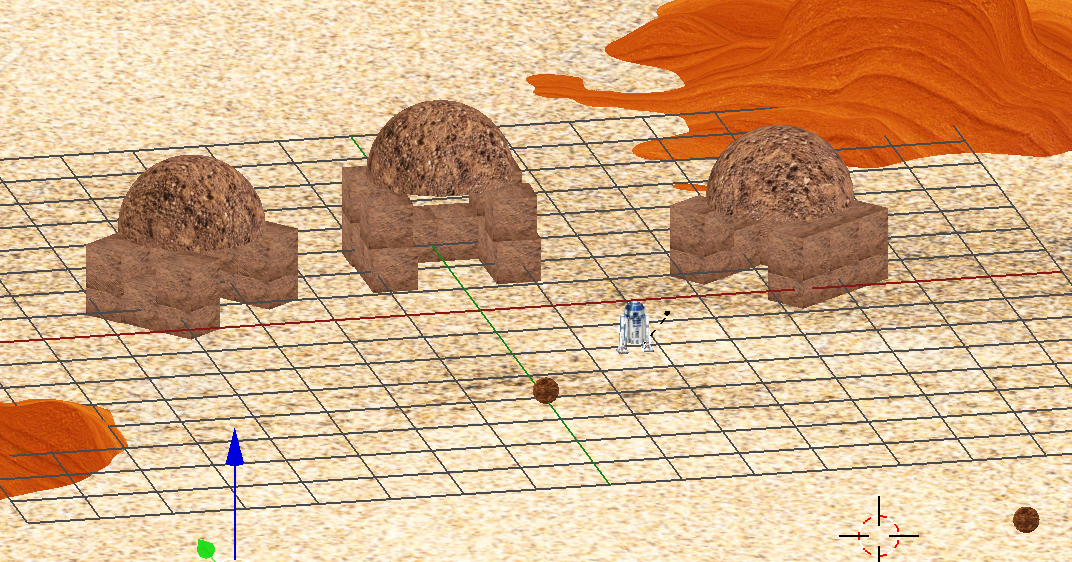
\includegraphics[scale=0.6]{./Capitulo1/Imagenes/tres.png}
		\caption{Modelo final.}
	\label{tres}
\end{figure} 



\section{Conclusiones finales}

La creaci�n de un entorno virtual complejo que se asimile a la realidad con mucho detalle es una tarea relativamente sencilla de realizar con Blender. Pese a que la aproximaci�n llevada a cabo por nosotros, dista mucho de la potencia total que el software puede desarrollar, hemos podido constatar como se pueden crear modelos y entornos muy realistas. 

Blender por tanto, pese a ser una herramienta de software libre, es una de las herramientas m�s potentes para la creaci�n de entornos virtuales, quedando esto confirmado a lo largo del desarrollo de la asignatura Entornos Virtuales, donde hemos abordado las opciones m�s interesantes y obtenido una perspectiva global de la potencia del programa.  

\clearpage
%---------------------------------------------------